\documentclass[12pt,letterpaper]{article}
\usepackage{fullpage}
\usepackage[top=2cm, bottom=4.5cm, left=2.5cm, right=2.5cm]{geometry}
\usepackage{amsmath,amsthm,amsfonts,amssymb,amscd}
\usepackage{lastpage}
\usepackage{enumerate}
\usepackage{fancyhdr}
\usepackage{mathrsfs}
\usepackage{xcolor}
\usepackage{graphicx}
\usepackage{listings}
\usepackage{hyperref}

\hypersetup{%
  colorlinks=true,
  linkcolor=blue,
  linkbordercolor={0 0 1}
}
 
\renewcommand\lstlistingname{Algorithm}
\renewcommand\lstlistlistingname{Algorithms}
\def\lstlistingautorefname{Alg.}

\lstdefinestyle{Python}{
    language        = Python,
    frame           = lines, 
    basicstyle      = \footnotesize,
    keywordstyle    = \color{blue},
    stringstyle     = \color{green},
    commentstyle    = \color{red}\ttfamily
}

\setlength{\parindent}{0.0in}
\setlength{\parskip}{0.05in}
\begin{document}






Foundations of Applied Math\\
 HW \#5 Geometric Similarity, Coding and Euler's Method
 Due Friday, Oct. 16 by 7 am

\textbf{Reminder} You need to turn in a .zipped folder that contains your .tex file, your image files, your python files, your Excel file(s), and the tex file must compile.
Rename the .tex file: HW5$\_$YourLastName.tex and call the folder which you will compress: HW4$\_$YourLastName


\begin{enumerate}

\item 
Recall that on Thursday Oct. 8, we ran this line in an example:
\begin{verbatim}
x=list(map(lambda x: x**3,x))
\end{verbatim}

\vspace{1em}
Recall also that in the HW \#4 solutions that are posted and that I went over on Friday, Oct. 9, I did this line in the first problem:

\begin{verbatim}
Pnext=lambda P,Q: P-.1*(Q-500) 
\end{verbatim}

\begin{enumerate}
\item[a)]  Why does the first example have a map command and the second example does not? Hint. What sort of input does each example take?
  The first command was to make a list which had a clear connection between the input indeces 
  and the output indeces. The second command, however, was a recursive commmand which depends
  on the previous values of P and Q, not on the values of the indeces of the array. 
\item[b)] Run the first example on a list of elements $2, 4, 6, 8$. Paste your python code here and also your output here. \\
  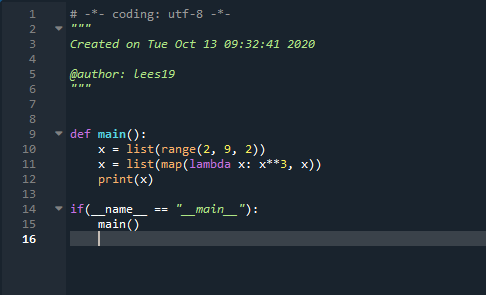
\includegraphics{number1bcode.png}\\
  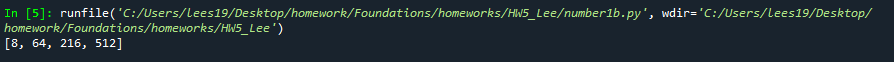
\includegraphics[scale = .7]{number1b.png}\\
  Python file is also included in number1b.py. 

\item[c)]  Run the second example on $P=100, Q=200$. Paste your python code here and also your output here.
\end{enumerate}
  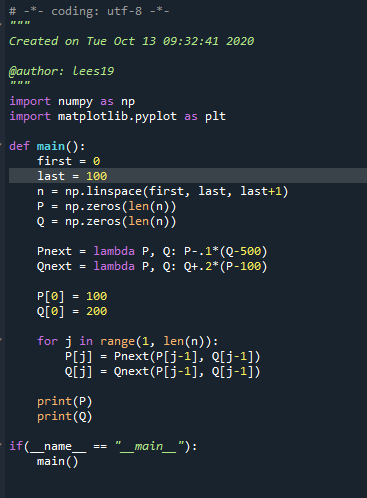
\includegraphics{number1ccode.png}\\
  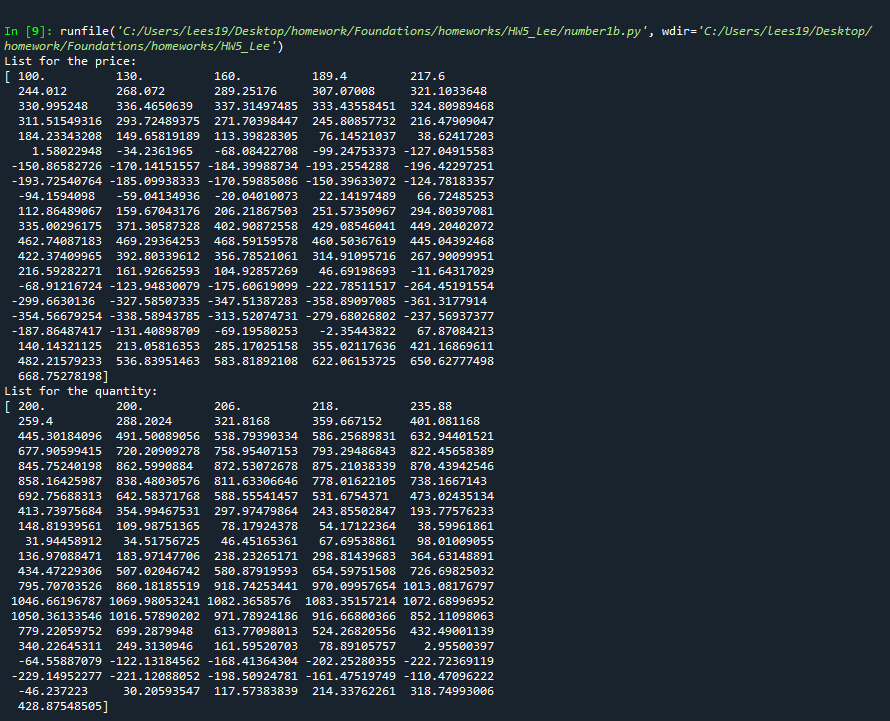
\includegraphics{number1c.png}
\pagebreak
\item Do 2.3) Projects \#3 on p. 94. Include your python code in your compressed folder and write your analysis here.

Just as we did in Project 2, we start with some assumptions:
\begin{gather*}
  E_{spent} \propto S\\
  E_{gain} \propto B\\
  E_{spent} = E_{gain} \\
  \rho = \frac{m}{V} \rightarrow V\rho = m \Rightarrow V \propto W
\end{gather*}

Then, since $E_{spent} \propto B$, $B \propto E_{spent}$. From there we see that 
B is proportional to W:  
\begin{gather*}
  B \propto E_{spent} \propto S \propto V^{\frac{2}{3}} \propto W^{\frac{2}{3}}\\
  B \propto W^{\frac{2}{3}}
\end{gather*}

Since $B$ is also proportional to $pV_{heart} \propto pV \propto pW$, we also find that $pW \propto W^{\frac{2}{3}}$
Dividing both sides by W, we find that $p \propto W^{-\frac{1}{3}}$. With this information, 
we use python to find the proportionality constant using our data set: \\

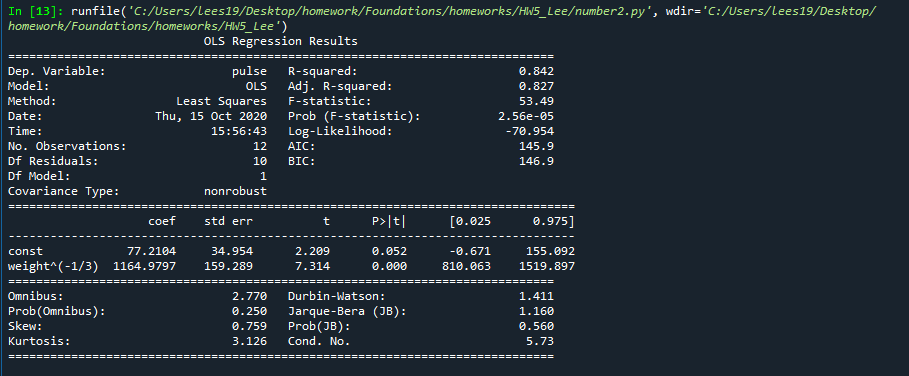
\includegraphics[scale = .7]{number2pval.png}

without forcing our y-intercept, and having a decent $R^2$ value, we fail to reject the 
null hypothesis that our y-intercept was zero. Therefore, we assume our data is proportional
and force the y-intercept to be zero: \\
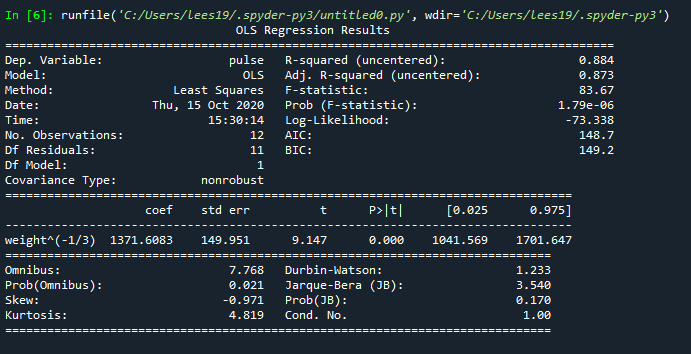
\includegraphics{number2.png}

From our python code, we find that our coefficient $k = 1371.6083$. Therefore, we find that 
$p = 1371.6083W^{-\frac{1}{3}}$\\

However, using this model, and looking at the percent errors for each of the weights, 
we find that the percent error is quite large for every single weight: \\
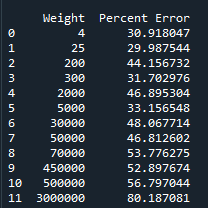
\includegraphics{number2error.png}

Therefore, we find that though our model is proportional, however the model we found 
does not fit our data very well. 

\item Given $$\frac{dP}{dt}=0.24P(11-P), P(0)=3$$ where $P$ is measured in 100's, answer the following.

\begin{enumerate}
\item[a)] Using Python, implement Euler's Method  with step size $h=0.1$ to approximate the solution for $P(2)$ and $P(6)$.  Write down the values for each. 
Also obtain a plot of the solution. Include your python file in your compressed folder and paste (use the includegraphics command) your plot here. \\
\emph{Solution.}\\

Using Euler's method and a step size of $h=.1$, we find that the approximation for P(2) and P(6) 
using python is approximately: $P(2) = 10.902853$ and $P(6) = 11.000000$. \\
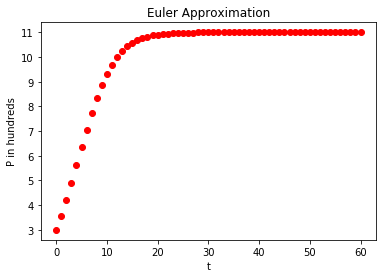
\includegraphics{number3.png}

The python file 'number3.py' is included. 

\item[b)] Do this in Excel. Include your Excel file in your compressed folder. Your work should match part a.
\\\emph{Solution.}

Using excel, we get the same values for $P(2) = 10.90285$ and $P(6) = 11.00000$ and obtain
a very similar looking graph as well: \\
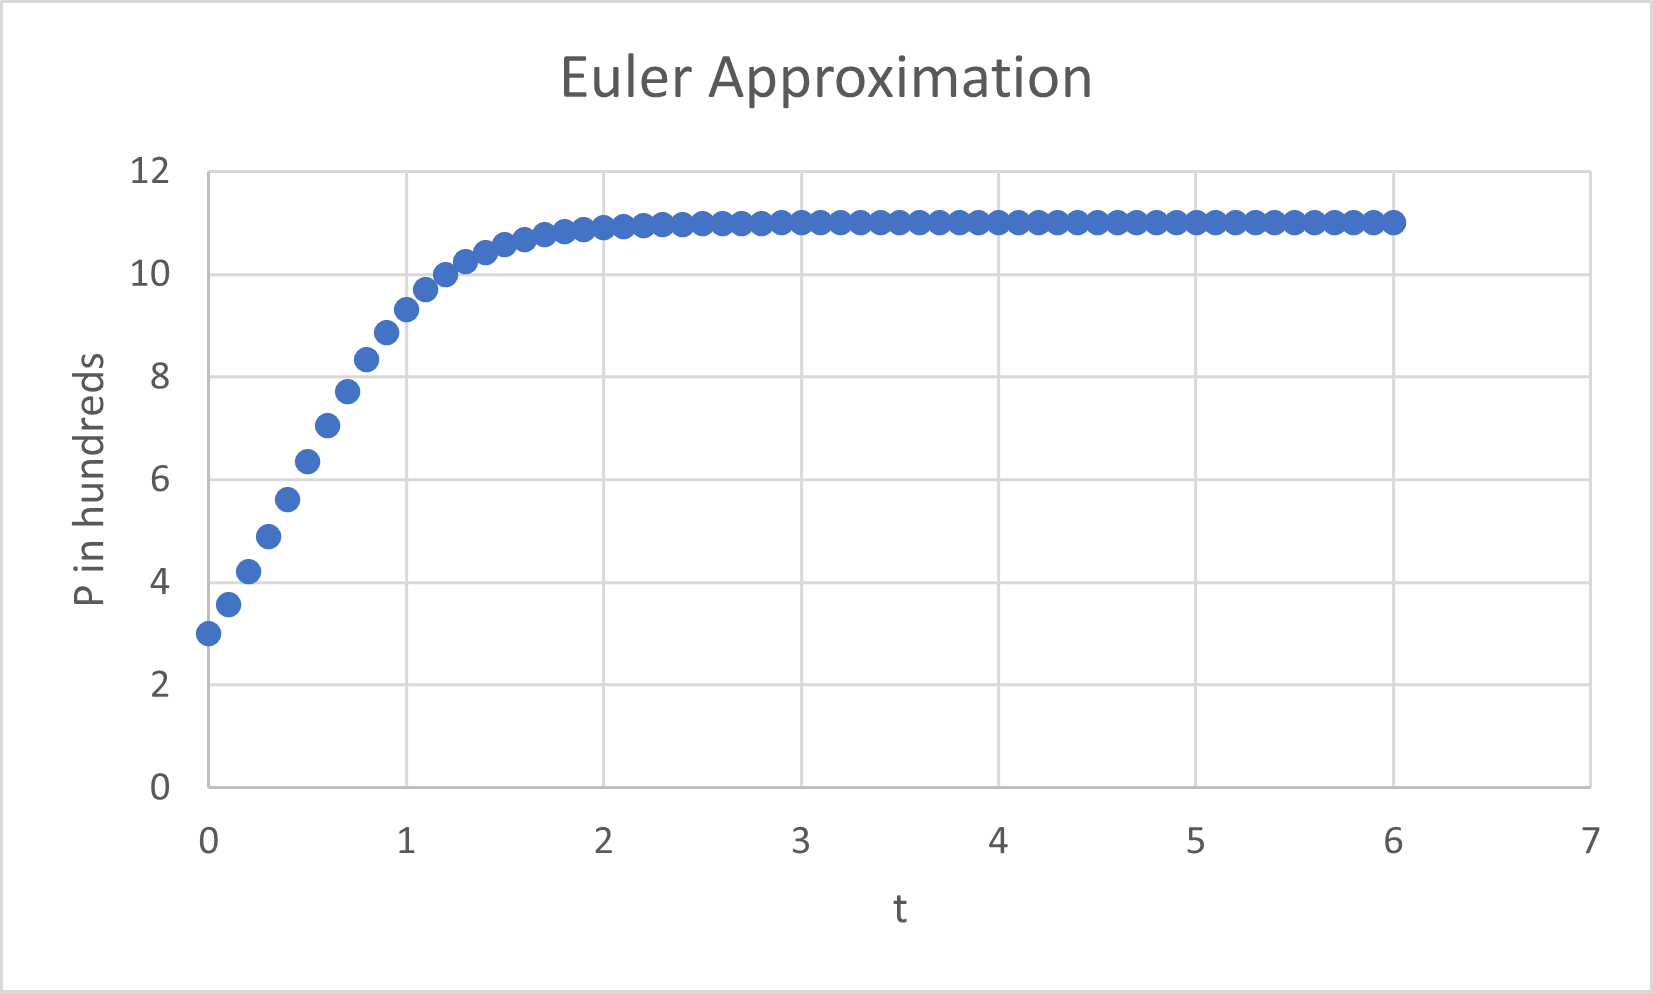
\includegraphics{number3excel.png}

The excel file 'number3.xlsx' is also included.

\end{enumerate}
\item  Given:


\begin{eqnarray*}
\frac{dR}{dt} &=& 0.65I(t)\\
\frac{dI}{dt}&=& -0.65I(t)+.0015I(t)S(t)\\
\frac{dS}{dt}&=& -.0015I(t)S(t)
\end{eqnarray*}

 Suppose that there are 2000 people in the population.  Suppose also that initially 6 people are infected. 
 \begin{enumerate}
 \item[a)] Using Python, implement Euler's Method  with step size $h=0.1$ \\
 \emph{Solution.}\\ 
 Python file 'number4.py' is included.  
\item[b)]  Do this in Excel. Include your Excel file in your compressed folder. Your work should match part a.\\
\emph{Solution.}\\ 
  Excel file 'number4.xlsx' is included. Using both excel and python, we see very similar results. \\
  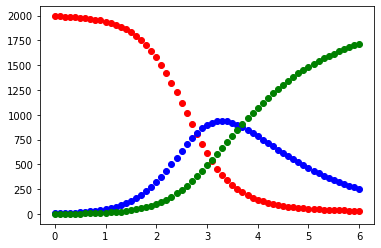
\includegraphics{number4py.png}\\
  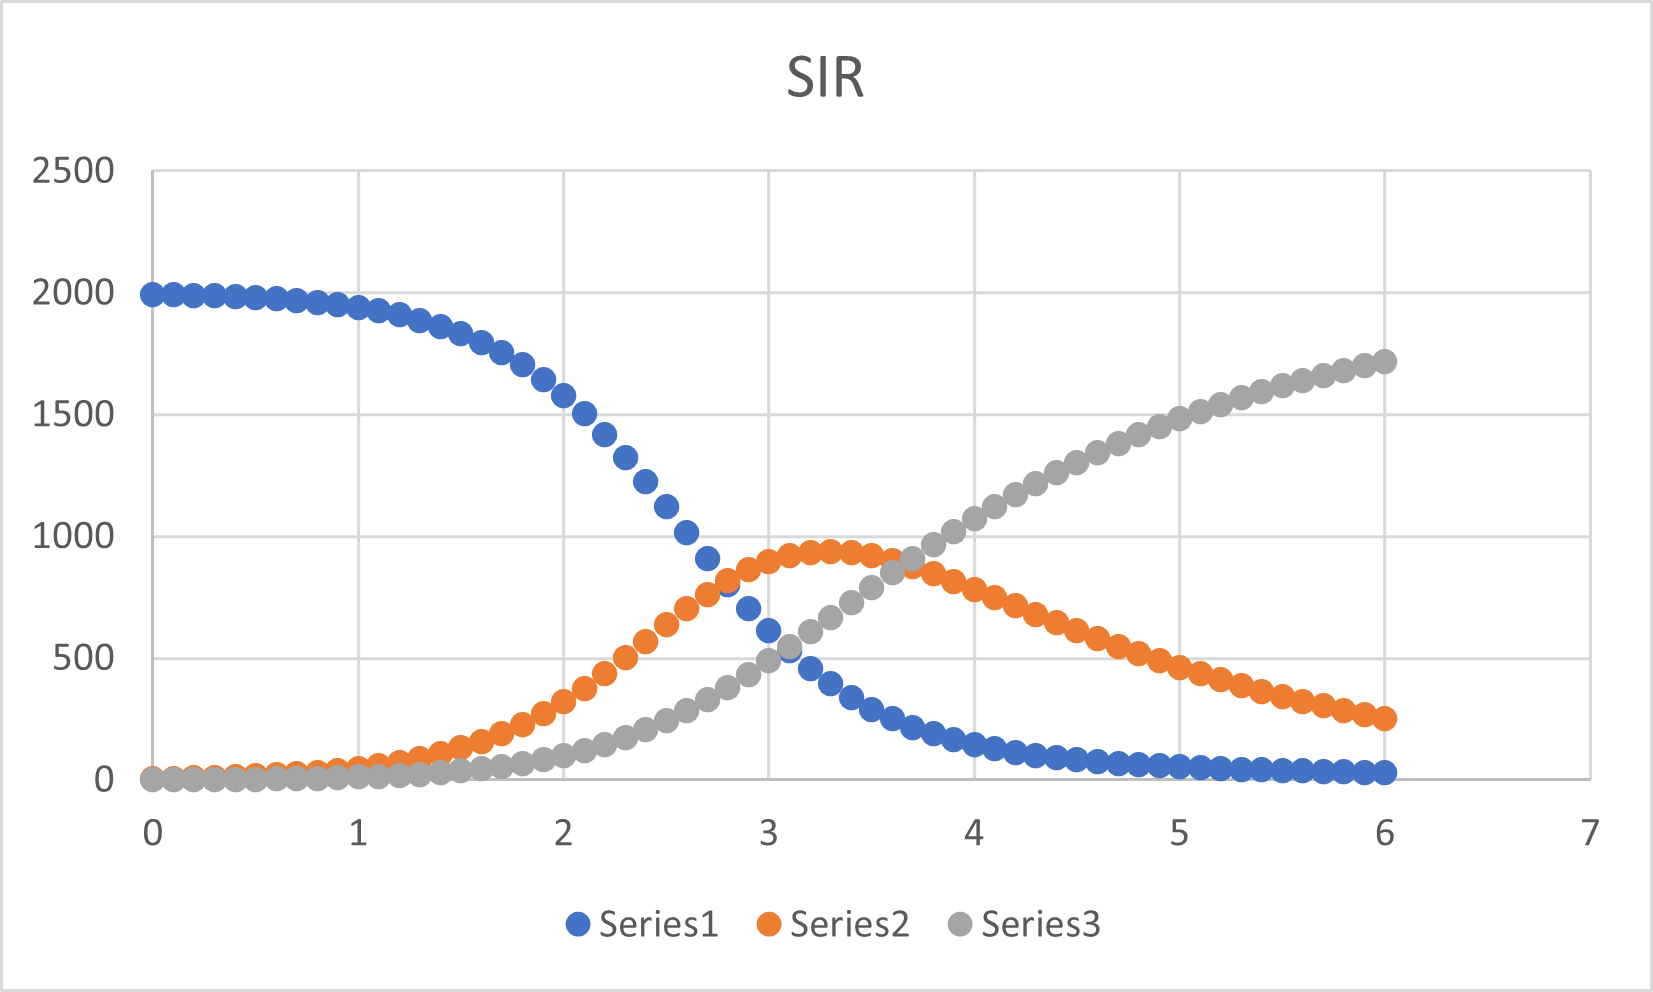
\includegraphics{number4excel.png}

  and looking at the actual values we see the actual numbers are also very similar : \\
  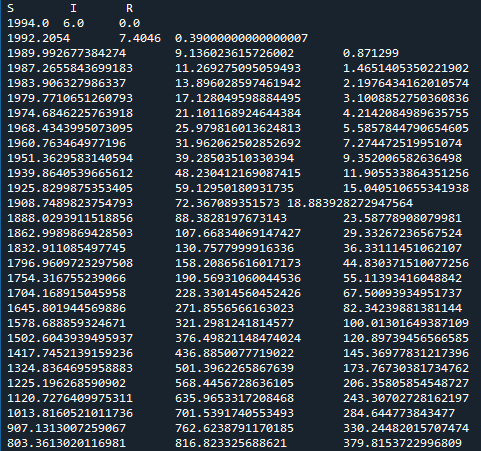
\includegraphics[scale = .9]{number4pygraph.png}
  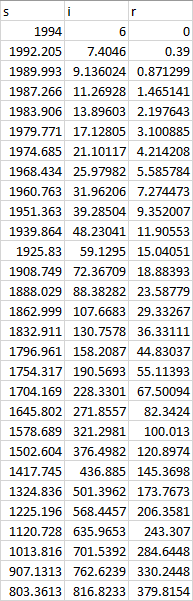
\includegraphics[scale = .68]{number4excelgraph.png}

\end{enumerate}

\item  Suppose squirrels and chipmunks compete for common resources in someone's backyard where they live all year long.


Let
\begin{itemize}
\item $C(t)$=the population of chipmunks at time $t$
\item $S(t)$= the population of squirrels at time $t$
\end{itemize}

Suppose also that:
\begin{itemize}
\item Chipmunks grow at a rate proportional to their population at any time.

\item Chipmunks decrease at a rate proportional to their interactions with each other.  This is called intracompetition and occurs because chipmunks are competing with each other for the same food and resources.

\item Squirrels grow at a rate proportional to their population at any time.

\item Squirrels  decrease at a rate proportional to their interactions with each other.  

\item Squirrels and chipmunks both compete for the same resources too. So this means that for squirrels and chipmunks they decrease at a rate proportional to the number of interactions they have with each other.  Assume that the proportionality constant is the same for both. 

\end{itemize}

\underline{ Write down a differential equation system that models this. }
\begin{gather}
  \frac{dC}{dt} = k_{1}C - k_{2}C^2 - k_{5}CS\\
  \frac{dS}{dt} = k_{3}S - k_{4}S^2 - k_{5}CS 
\end{gather}


\end{enumerate}


\end{document}